
\section{Requirements}

\subsection{Who Will Be Served}

The main drive for this completion of this project is Saurabh Chakravarty, our client. By iterating over his feedback, we are treating him as the eventual end user. Eric Williamson is also working with Saurabh as an additional client for the project and a potential end user.  Theoretically there is room for expansion when it comes to future users. If we are successful in “predicting” the stock market, there is potential for our work to be used for monetary gain, but no plan is in place at the current time. 

Automated stock trading is a rapidly developing research area. Our paper will help to further expand this research. Its availability on VTechWorks will allow future researchers to expand upon our work.  As evidenced by our group's use of earlier work done at Virginia Tech through CrowdIQ we can provide an exceptional roadmap to jump start others' forays into utilizing microblogging data as predictive input.  

Formally there are no current plans for extended support. As opposed to other potential projects in this class ours is more conceptual/research based. Hopefully, the ability to reference our research as we previously described will result in its future use.

\subsection{Scenarios Served}

\begin{table}
  \centering
  \begin{tabular}{ | r | l | }
    \hline
    Symbol & Name \\ \hline
    \texttt{\$APPL} & Apple Inc. \\ \hline
    \texttt{\$GILD} & Gilead Sciences Inc. \\ \hline
    \texttt{\$KNDI} & Kandi Technologies Group Inc. \\ \hline
    \texttt{\$MNKD} & MannKind Corporation \\ \hline
    \texttt{\$NQ} & NQ Mobile Inc. \\\hline
    \texttt{\$PLUG} & Plug Power Inc. \\\hline
    \texttt{\$QQQ} & PowerShares QQQ Trust, Series 1 (ETF) \\\hline
    \texttt{\$SPY} & SPDR S\&P 500 ETF Trust \\\hline
    \texttt{\$TSLA} & Tesla Inc. \\\hline
  \end{tabular}
  \caption{Baseline Stocks}\label{tab:stocks}
\end{table}

The initial scenario we are focusing on is the set of trading days from 2014 on the stocks shown in Table~\ref{tab:stocks}. This set of historical data is used to compare our results to a baseline. This will allow us to iterate through different trading methods much more quickly as we will be able to retrieve the stock pricing for this data once and store it locally for quicker and easier access.

Next, testing will be done on other timeframes of historical data and on more stocks than the baseline. The framework to acquire the data for this time period will be facilitated by the same tool used to acquire the new data. This will allow us to ensure that our trading method is not created just to specifically fit the data from 2014. This additional testing comes at a much lower cost than going straight to real time testing as it will be quicker and much of the implementation overlaps from the baseline set. 

The final scenario will be real time testing, but will differ slightly based on trading strategy. For example our first baseline strategy trades only once a day at opening, but a future strategy will most likely trade multiple times throughout the day. With proper implementation this change in timing will be a simple change of program parameters. This final scenario would be the closest model to any real life implementation of a program similar to ours. 

\subsection{Data To Be Processed}

\begin{figure}
  \centering
  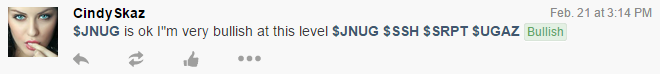
\includegraphics[width=5in]{stocktwits}
  \caption{Example microblog post from StockTwits}\label{fig:stocktwits}
\end{figure}

As mentioned before the main dataset involved in micro-blogging entries from the web site StockTwits. These are more colloquially referred to as just tweets. Each tweet will contain a stock symbol at the front as a way to determine what stock the user is talking about (see Figure~\ref{fig:stocktwits}). Some tweets will also contain a tag referring to the tweet as either bullish or bearish. After data classification all the tweets without tags will be assigned a tag.

The initial data set will focus on nine stocks, shown in Table~\ref{tab:stocks}, for the year 2014. However, the scope will be expanded to other time frames and to eventually real-time acquisition of micro-blogging data and same day trading.

Some of our ideas for trading will possibly expand our dataset to other possible areas of sentiment analysis. We have found research using financial surveys and other reports as supplementary areas of sentiment to adjust the overall sentiment of a stock.

\subsection{Existing Code Base}

Saurabh and Eric have provided us with some code that will help implement the classification. This code is in the Scala general-purpose programming language. Due to this code already being created we have decided to do the rest of the program in Scala as well and will be storing in on a public GitHub repository.

We will also make use of previous implementations of chosen machine learning algorithms (specifically those provided in the Spark.ML library). This will allow us to save time by not creating anything that already exists.

%%% Local Variables:
%%% mode: latex
%%% TeX-master: "../report"
%%% End:
